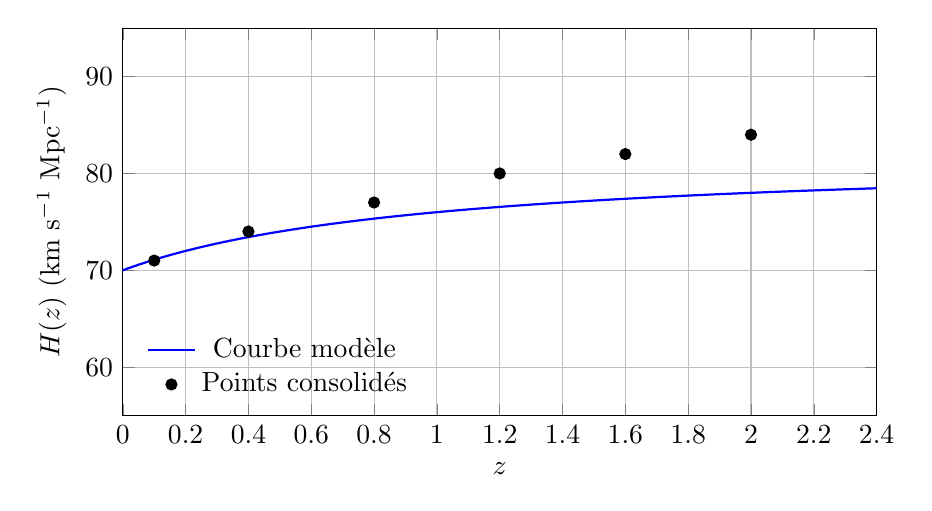
\begin{tikzpicture}
\begin{axis}[
    width=0.92\linewidth,
    height=6.5cm,
    xlabel={$z$},
    ylabel={$H(z)$ (km s$^{-1}$ Mpc$^{-1}$)},
    xmin=0, xmax=2.4,
    ymin=55, ymax=95,
    grid=both,
    legend style={at={(0.02,0.02)},anchor=south west,draw=none,fill=none},
]
\addplot[blue,thick,samples=100,domain=0:2.4] {70 + 12*x/(1+x)};
\addlegendentry{Courbe modèle}
\addplot[only marks,mark=*,black] coordinates {
    (0.1,71)
    (0.4,74)
    (0.8,77)
    (1.2,80)
    (1.6,82)
    (2.0,84)
};
\addlegendentry{Points consolidés}
\end{axis}
\end{tikzpicture}